\documentclass{standalone}

\usepackage{pgfplots}
\pgfplotsset{compat=1.15}

\begin{document}

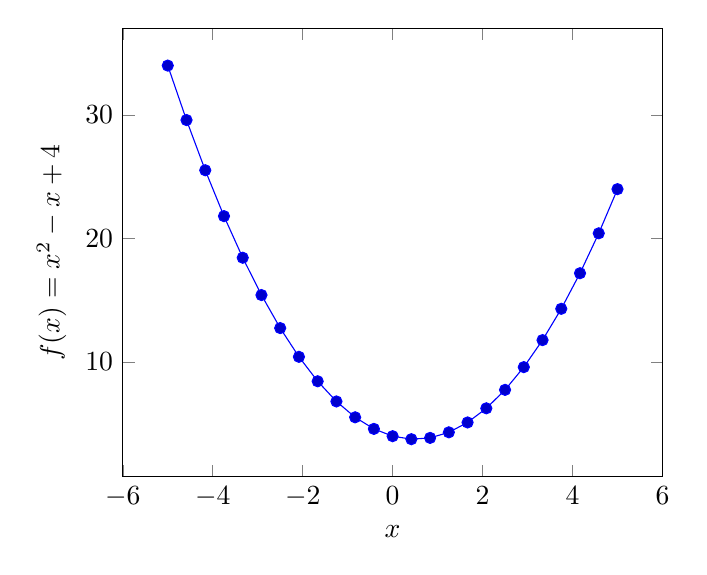
\begin{tikzpicture}
  \begin{axis}[ 
    xlabel=$x$,
    ylabel={$f(x) = x^2 - x +4$}
  ] 
    \addplot {x^2 - x +4}; 
  \end{axis}
\end{tikzpicture}

\vspace{1 in}

\begin{tabular}{|c|c|}
\hline 
$x$ & $y$ \tabularnewline
\hline 
\hline 
$3$ & $5$ \tabularnewline
\hline 
 & \tabularnewline
\hline 
 & \tabularnewline
\hline 
 & \tabularnewline
\hline 
 & \tabularnewline
\hline 
\end{tabular}

\end{document}
